\chapter{Discussion}
In the analysis of the state constraint, we introduce a Barrier Lyapunov Function and use the proposition 2 to show the feasibility of agent $z_k$. However, this method is yet still not proven under a mathematical analysis. There might be some sufficient and necessary conditions that must be fulfilled. In this chapter, we discuss about this challenge with more details and propose related future work in the conclusion. \\ \\
%\section{Problem Review}
\noindent We introduce the coverage control in one dimension to demonstrate intuitively the concept of proposition 2. Figure \ref{fig:Schematic_1D} depicts the schematic of the 1D coverage problem, in which we have two agents trying to approach the center masses. Intuitively, the boundary of the Voronoi cell between these 2 agents is the perpendicular bisector, which divides the coverage region into two bounded sub-regions. Obviously, the center mass is always the middle point of one region.
\begin{figure} [!h]
	\centering
	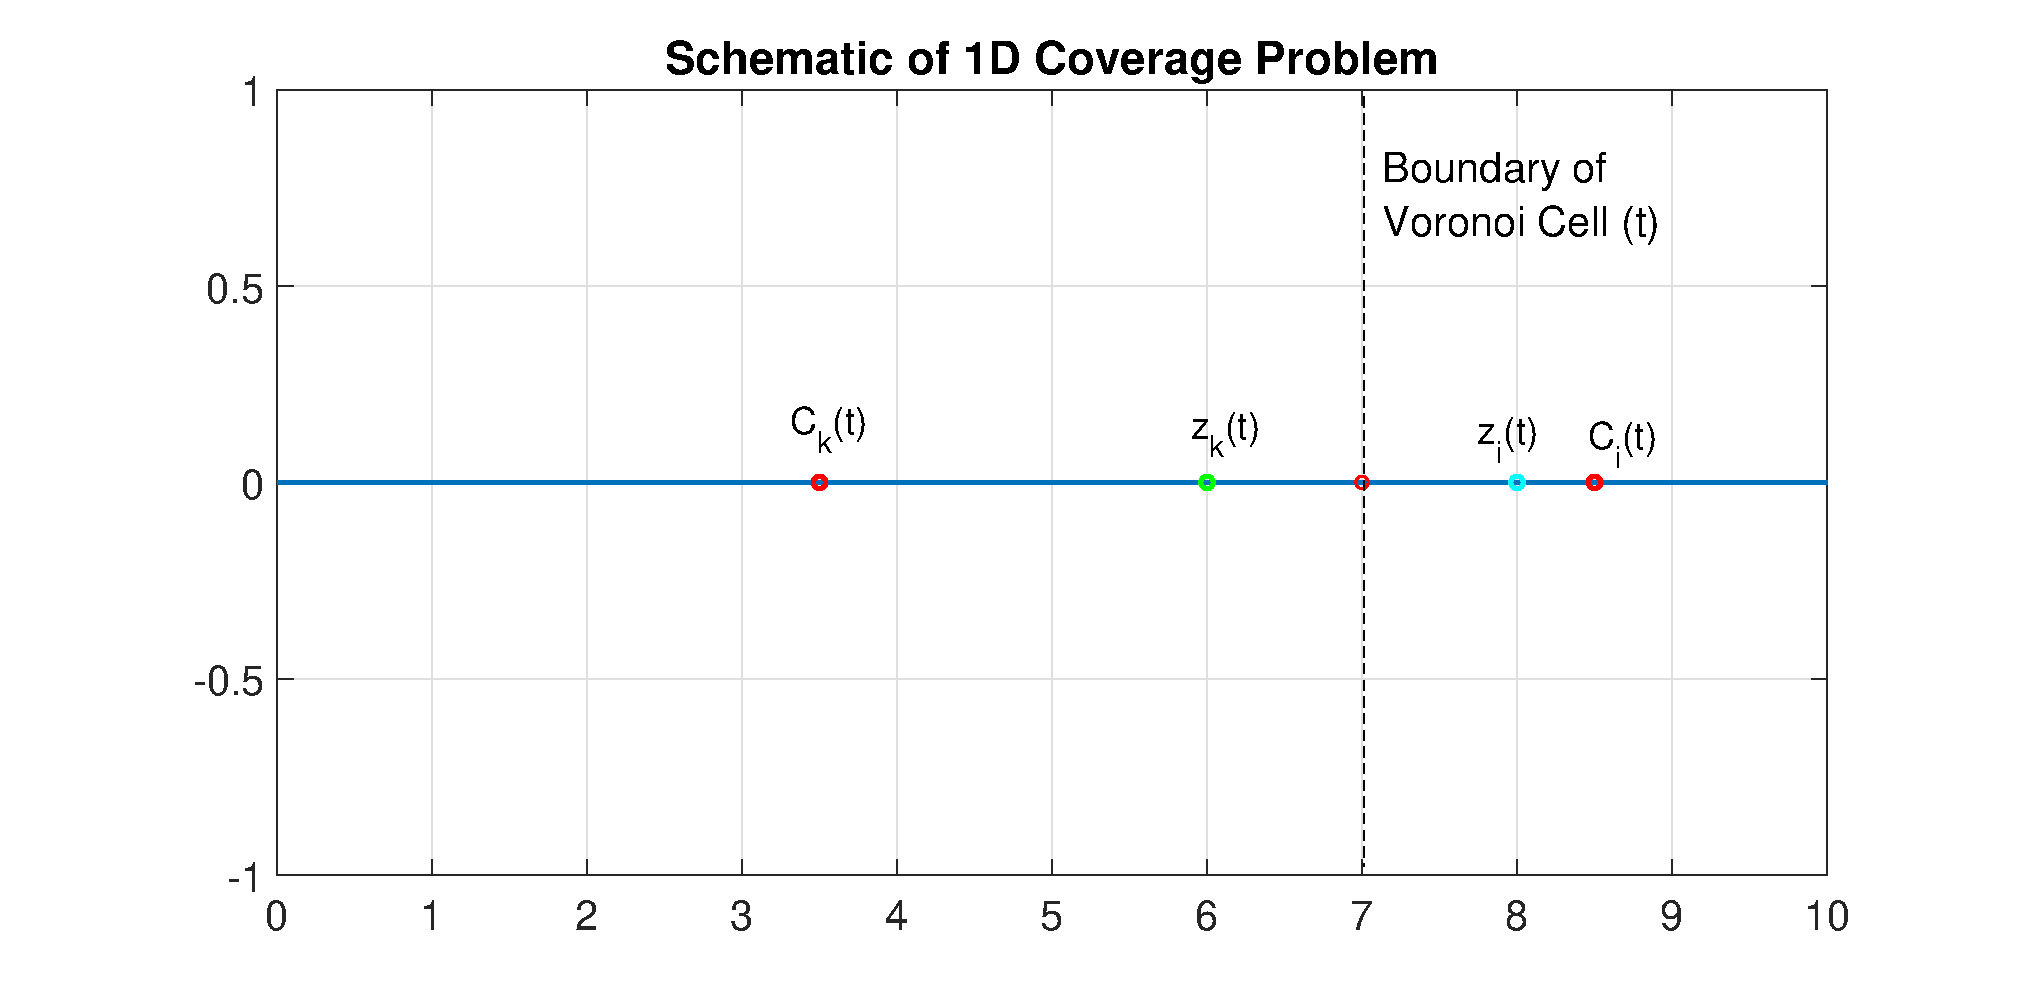
\includegraphics[width=1\linewidth]{Schematic_1D_Line}
	\caption{Schematic of 1D Coverage}
	\label{fig:Schematic_1D}
\end{figure}

\noindent Since the boundaries are fixed, the center mass $C_k$ depends only on the position of two agents. From the BLF in 2D Coverage Problem, we apply it for the 1D scenario.
\begin{equation}
V_k(Z(t)) = \displaystyle\sum_{j}^{} ln(\frac{b_j - a_jC_k(t)}{b_j - a_{j}z_{k}(t)})^2
\end{equation} 
where $j$ denotes the boundaries. From the definition of our Barrier Lyapunov Function, it has the following properties: \\
$\bullet$ $C_k(Z)$ is always the local optimum of the BLF. \\
$\bullet$ $C_k(Z)$ and $V_k(Z)$ are always well defined if the agents are always inside the interior of the coverage region. \\
There exists a descent direction of $V_k(Z)$ related to $z_k$, we use the convexity of the region to show that $z_k$ is still feasible if it follows this direction. Figure \ref{fig:BLF_2D_1} illustrates the descent direction of $V_k$. Note that the plot shows the contour of $V_k(Z)$, which depends on the position of both two agents and the green point is a vector notation that represents the position of two agents at any time.
\begin{figure} [!h]
	\centering
	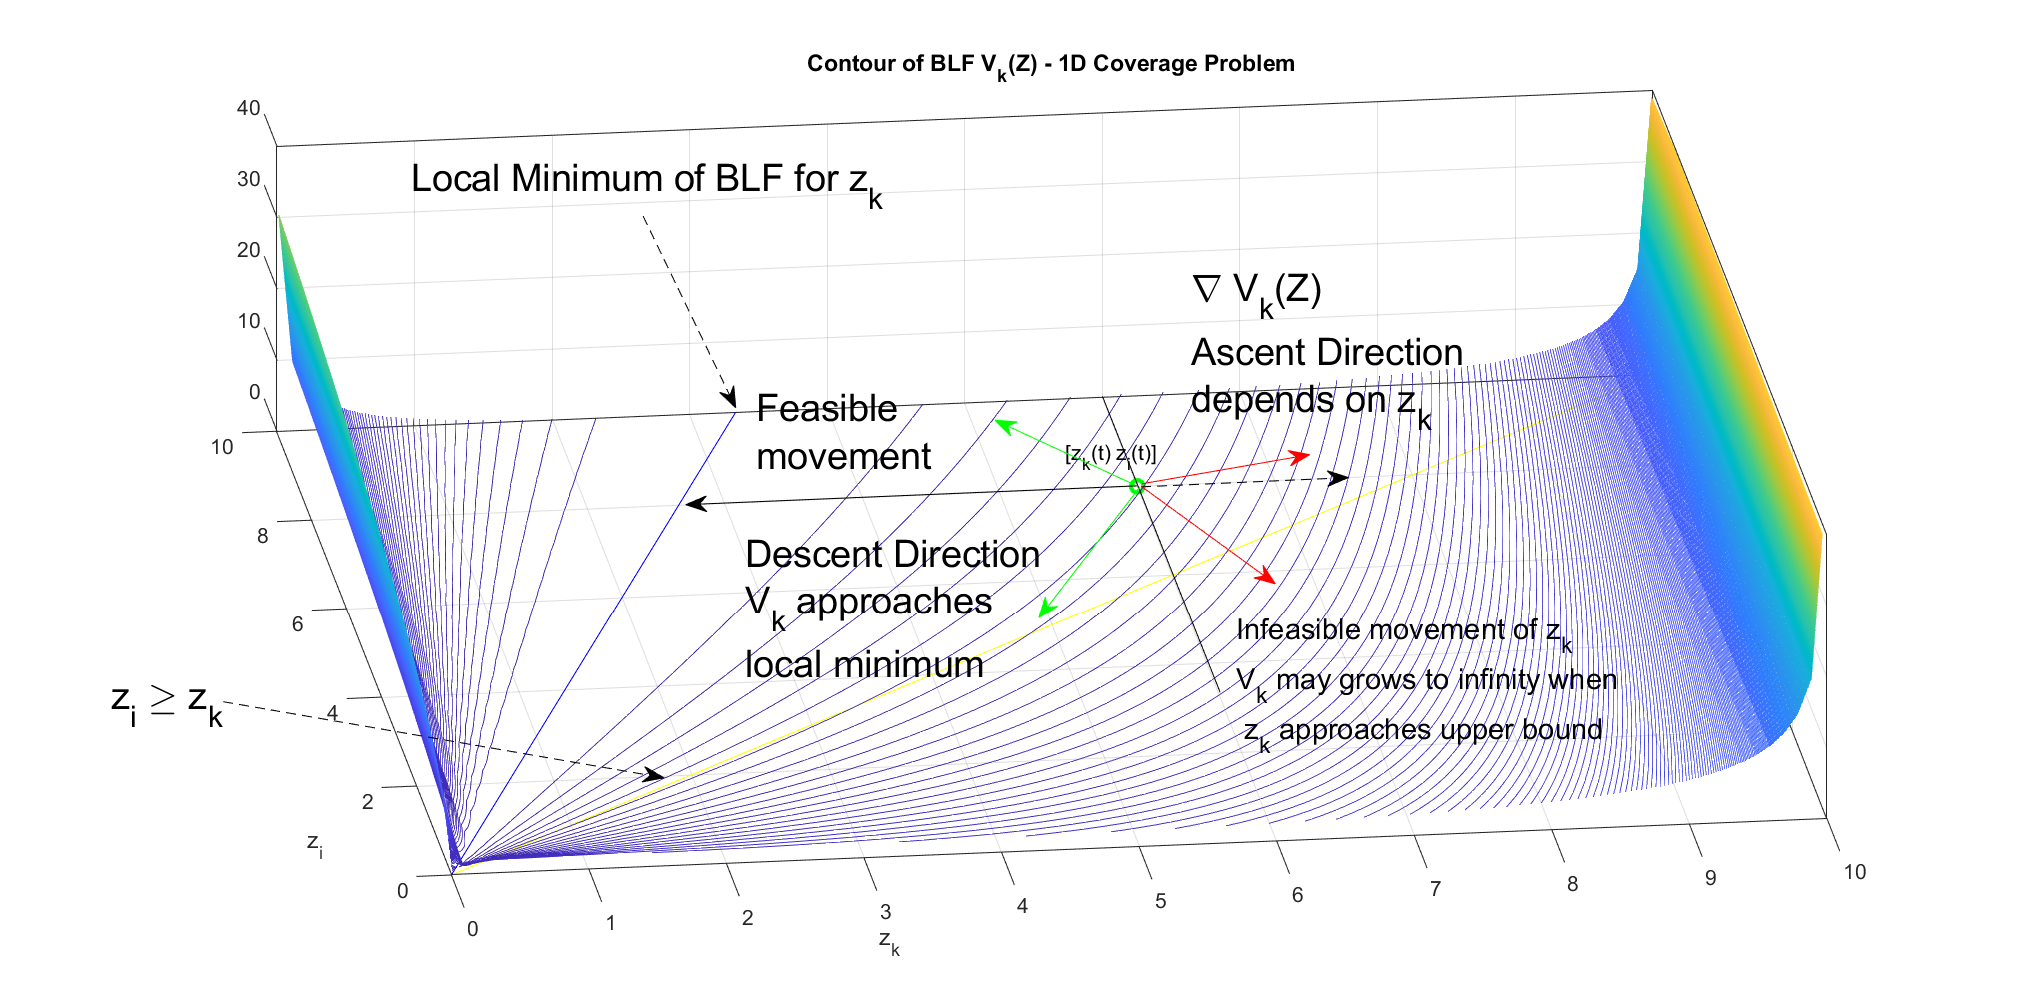
\includegraphics[width=1\linewidth]{Contour_1D_Coverage_Problem_BLF_zoom}
	\caption{Contour of BLF in 1D Coverage Problem}
	\label{fig:BLF_2D_1}
\end{figure}

\begin{figure} [!h]
	\centering
	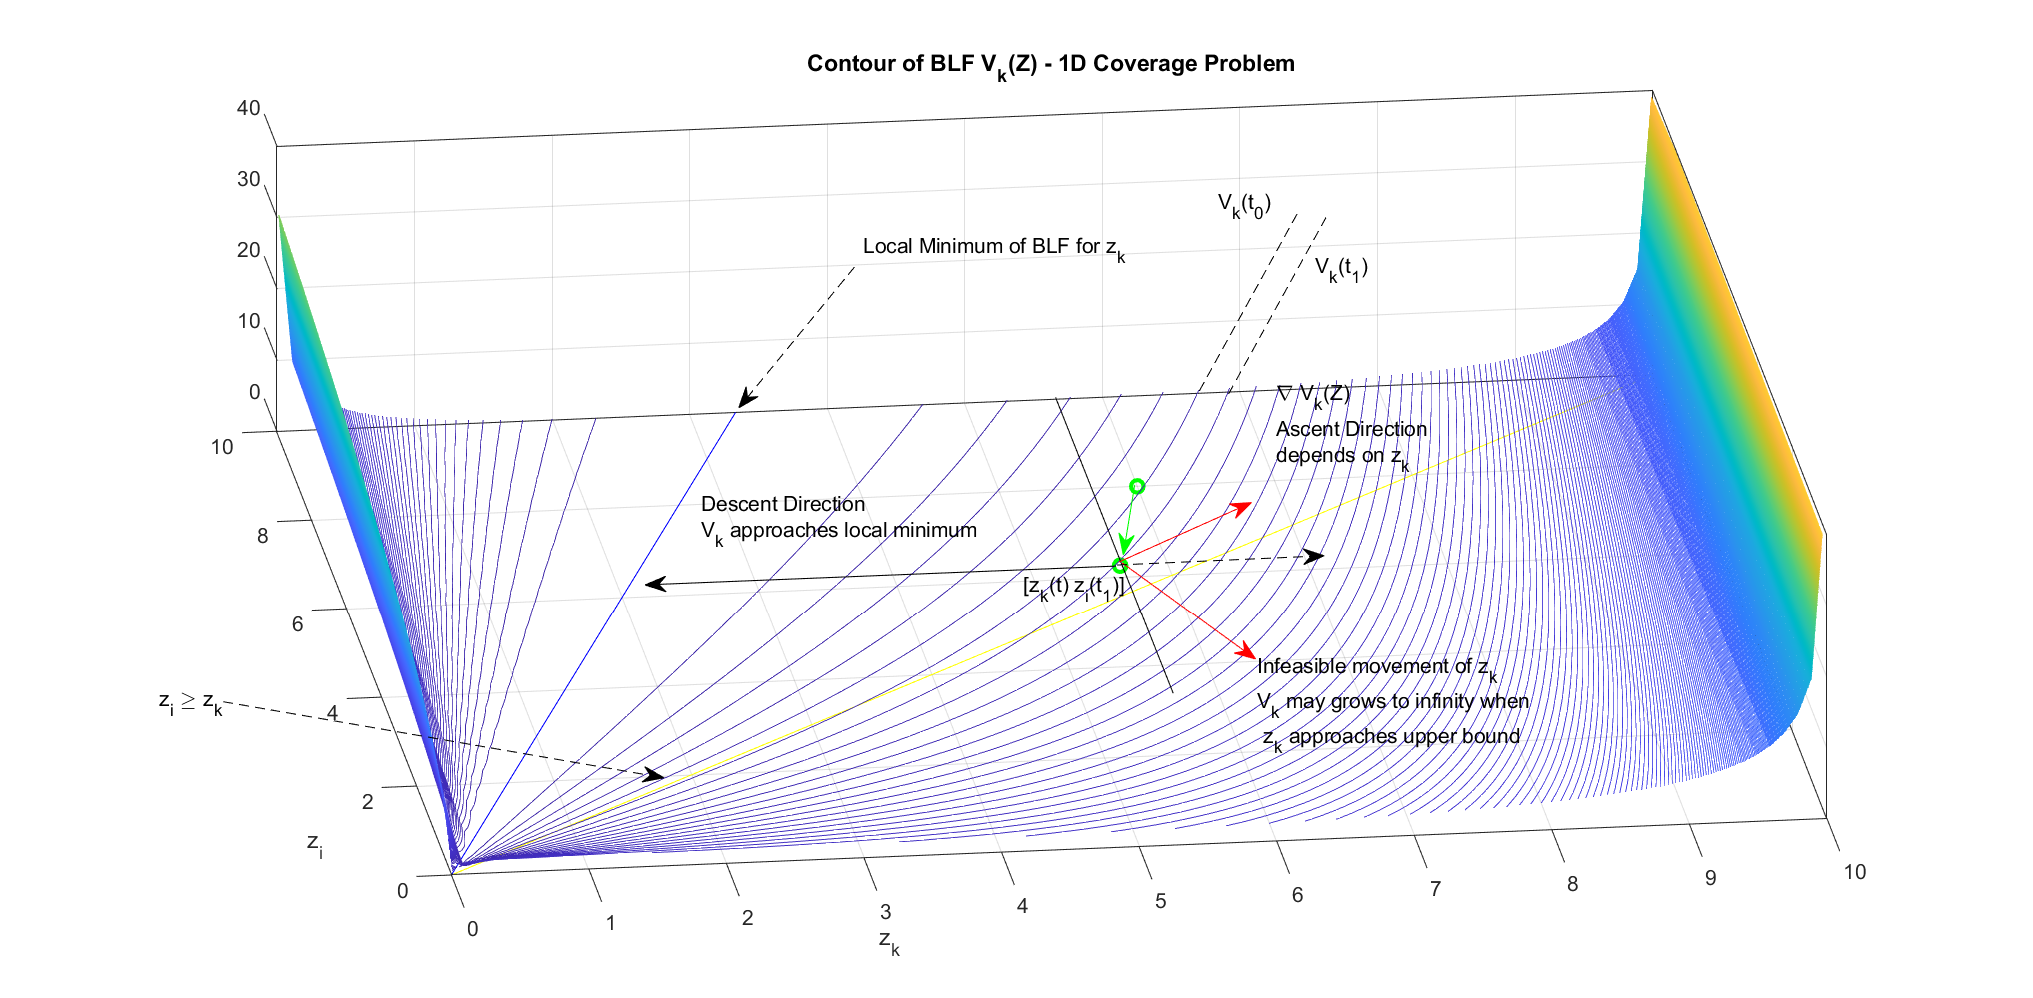
\includegraphics[width=1\linewidth]{BLF_1D_Coverage_Contour_Time_Evolution}
	\caption{Feasibility of Agent k in 1D Coverage Problem}
	\label{fig:BLF_2D_2}
\end{figure}
\noindent We observe that if $z_k$ always approaches $C_k$ by following the descent direction, it maintains inside the coverage region because the region is convex and $C_k$ is the local minimum of BLF. \\
Figure \ref{fig:BLF_2D_2} shows the time evolution of $z_k$. Even $z_k$ (x Axis) moves in the feasible direction, the BLF can still increase because the neighbor (y Axis) moves in the ascent direction related to $z_i$. Consequently, using this BLF alone can not solve the problem of coverage control because of the non-negative time derivative. However, what we need is just a feasible direction that guarantee the state constraints, and as long as all of the virtual masses keep moving, they converge to the set of centroidal Voronoi asymptotically. 



